\subsection{Topological Fluctuations within Quark-Gluon Plasma}
\label{Sec:Exotica}

It has been known for decades that topological effects play an
important role in determining the structure of the vacuum in
non-Abelian gauge theories\cite{Belavin:1975fg}.  In QCD, fluctuations
that change the topology of the non-Abelian gauge fields are at the
same time fluctuations that create an imbalance of chirality.
Recently, considerable interest has been generated by the possibility
of exploring experimental signatures of such fluctuations in the hot
QCD matter produced in relativistic heavy ion collisions.  A key
observation is that the incredibly strong magnetic field that is
generated in off-center heavy ion collisions, together with the chiral
anomaly in QCD and the fluctuations in chirality, can produce a Chiral
Magnetic
Effect~\cite{Kharzeev:2007tn,Kharzeev:2007jp,Fukushima:2008xe,Hirono:2014oda}
in which an electric current flows along (for one sign of the
chirality fluctuation) or opposite to (for the other sign of the
chirality fluctuation) the direction of the magnetic field, resulting
in a separation of particles with opposite electric charge in a
direction perpendicular to the reaction plane of the collision, while
particles with the same electric charge show a preference for ending
up in the same hemisphere.
\begin{figure}[!htp]
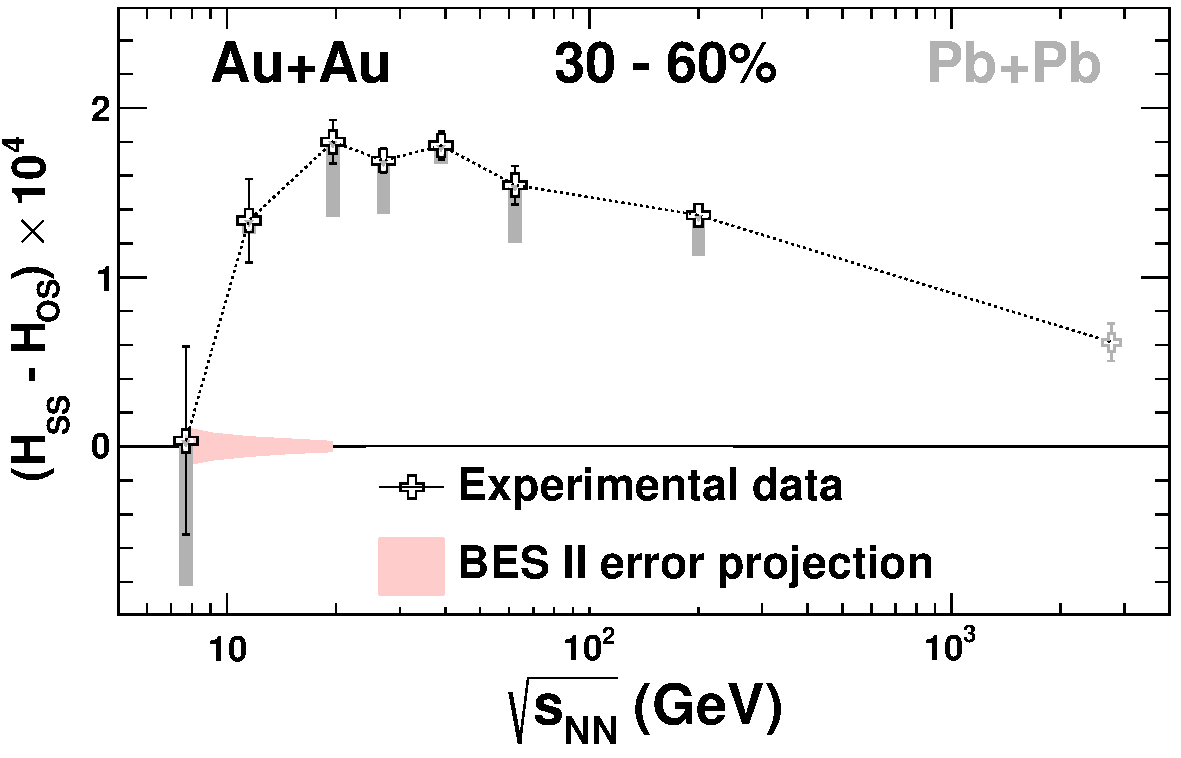
\includegraphics[width=\textwidth]{fig/CMEfromBES.pdf}
\caption[Charge separation results from STAR and ALICE]{Collision energy dependence of the charge separation
  correlation $H$ difference between same-sign (SS) and opposite sign
  (OS) pairs in mid-central (30-60\%) \AuAu\ collisions by RHIC\cite{Adamczyk:2014mzf}
  ($\sqrt{s_{NN}}= 7.7 - 200$ GeV) and Pb+Pb collisions at LHC\cite{Abelev:2012pa}
  ($\sqrt{s_{NN}}= 2.76$~TeV). The hatched band represents the
  estimated statistical errors that will be obtained in BES II
  measurements at RHIC.}
\label{Fig:CME}
\end{figure}

Such an effect has been observed by using the three-point correlator
method~\cite{Voloshin:2004vk} to extract event-plane dependent charge
correlations in \PbPb\ collisions at the LHC~\cite{Abelev:2012pa} and
at a variety of collision energies at
RHIC\cite{Abelev:2009ac,Abelev:2009ad,Adamczyk:2014mzf}.  Conclusively
establishing that these observations result from the CME would be an
important advance in our ability to study experimentally the
topological phase structure of QCD.  In addition, the effect itself
can be used to study the properties of the medium created in the
collisions. Since the CME requires the formation of QGP, {\it e.g.}
the restoration of the chiral symmetry~\cite{Hirono:2014oda}, one
would expect that at sufficiently low energy, the QCD related
correlations should disappear. This is precisely what is observed in
$\sqrt{s_{NN}}$=11.5 GeV \AuAu\ collisions~\cite{Adamczyk:2014mzf}, as
shown in Figure~\ref{Fig:CME}.

\begin{figure}[!htp]
\includegraphics*[width=0.9\textwidth]{fig/CVEfromSTAR}
\vspace{-1.5cm}
\caption[Baryon separation as a function of collision centrality from STAR]{Baryon separation shown as a function of collision centrality
  from $\sqrt{s_{NN}}=200$ GeV Au+Au collisions. Circles and triangles
  represent the data for the same-baryon-number and
  opposite-baryon-number correlations, respectively.  Error bars are
  statistical only. Taken from \cite{Zhao:2014aja}.}
\label{Fig:CVE}
\end{figure}
The same physical mechanism that produces the Chiral Magnetic Effect
in the presence of a magnetic field $\vec B$ can also produce a Chiral
Vortical Effect (CVE) in the presence of external angular momentum
$\vec L$~\cite{Kharzeev:2010gr}.  While high energy nuclear collisions
produce the strongest known magnetic fields $\sim 10^{18}$
gauss\footnote{The magnetic field at the surface of magnetars is on
  the order of $10^{15}$ gauss, several orders of magnitude lower than
  the field strength in high-energy nuclear collisions.}, these fields
are largest at the very beginning of the collision and decay away on a
timescale that is controlled by the electric conductivity of the
matter produced in the
collision~\cite{Tuchin:2013ie,McLerran:2013hla,Gursoy:2014aka}.
Angular momentum, on the other hand, is conserved meaning that if the
plasma is created with nonzero angular momentum this remains.  If
topological fluctuations and the associated chirality fluctuations do
have observable effects in high energy nuclear collisions, then in
addition to the charge separation along the external magnetic field in
the CME one would expect baryon number separation along the (same)
direction of the external angular momentum.  The first measurements of
observables that receive a contribution from any CVE were reported
recently for \AuAu\ collisions at 200 GeV for proton (anti-proton) and
Lambda (anti-Lambda) pairs~\cite{Zhao:2014aja}, as shown in
Figure~\ref{Fig:CVE}.  The figure indicates a preference for proton
and Lambda pairs, as well as antiproton and anti-Lambda pairs, to be
found in the same hemisphere.

%Both the CME or CVE are consequences of the fundamental symmetries of QCD. 
%Therefore the underlying physics is not limited to high energy nuclear collisions, but should be expected in other strongly interacting systems.

The topological fluctuations that drive the CME and CVE in QCD have
analogues in other gauge theories and arise in other contexts.  For
example,
%within the frame of standard model, 
it has been argued that if an electron chirality imbalance exists in
the weakly coupled electroweak plasma at temperatures thousands of
times hotter than those achieved in heavy ion collisions, this may be
responsible for the primordial magnetic fields in the early
Universe~\cite{Joyce:1997uy}.  Furthermore, the same kinds of
topological fluctuations that make a chirality imbalance in the
quark-gluon plasma can make a baryon number imbalance in the much
hotter electroweak plasma, meaning that if these fluctuations were in
some way biased they could be responsible for the
matter-over-antimatter excess in the Universe.  In a third context,
the CME has been realized in condensed matter physics in a
(3+1)-dimensional structure called a Weyl semimetal due to the chiral
anomaly~\cite{Wan:2011aa} and in other systems as reported in
Ref.~\cite{Perks:2012aa}.
%Recently, the CME has been successfully introduced
%into event-by-event chiral magnetohydrodynamics simulations~\cite{Hirono:2014oda}, which marks a milestone for quantitative understand of such basic QCD symmetry effects in high-energy nuclear collisions. 
  
As can be seen from Figure~\ref{Fig:CME}, the error bars in the current
data are still large, especially in the lower energy region. As a
result, it is not yet possible to systematically investigate these
phenomena as a function of energy, nor is it possible to
determine the exact collision energy where the CME disappears. The
planned BES-II program at RHIC, discussed in Section~\ref{Sec:CP},
will provide high statistics data for CME and CVE studies in
\AuAu\ collisions at energies below 20~GeV. The estimated errors are
shown as the shaded bar in Figure~\ref{Fig:CME}.  With such
measurements, along with the planned dilepton measurements, we may
expect to gain significantly improved quantitative understanding of
the chiral properties of hot QCD matter at nonzero baryon density.
 



%---==========================================================================================================
